\section{Aufbau und Durchführung}
\subsection{Aufbau}
\label{sec:Aufbau}

Das im vorliegenden Versuch verwendete Michelson-Interferometer ist in Abbildung \ref{abb:2} schematisch dargestellt.
\begin{figure}[H]
  \centering
  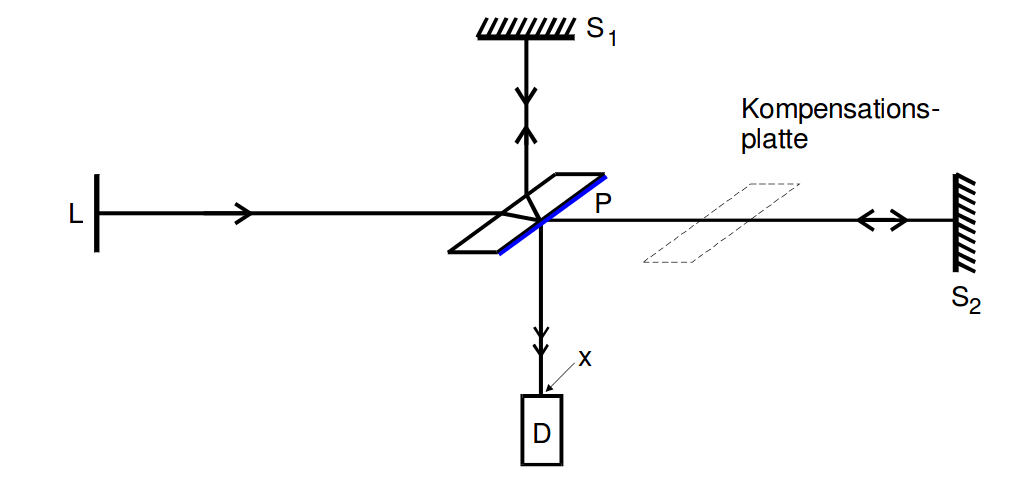
\includegraphics[height=4cm]{ressources/aufbau1.png}
  \caption{Schematischer Aufbau eines Michelson Interferometers. \cite{skript}}
  \label{abb:1}
\end{figure}

\subsubsection{Grundlegender Aufbau der Michelson-Interferometers}
Ein Lichtstrahl, welcher hier durch einen Laser erzeugt wird, wird vom Ort $L$ zu einem halbdurchlässigen Spiegel am Ort $P$ gelenkt.
Durch die Eigenschaften des halbdurchlässigen Spiegels wird der Strahl nun entweder zum Spiegel $S_1$ reflektiert oder zum Spiegel $S_2$ durchgelassen.
Beide Strahlen werden nun am Spiegel jeweiligen reflektiert, der erste Strahl kann nun wieder eine Reflexion an $P$ erfahren oder durchgelassen werden: In diesem Fall endet der Lichtstrahl am Detektor $D$.
Beim zweiten Strahl, der vom Spiegel $S_2$ kommt, können ebenfalls beide Fälle auftreten.
Im Falle einer Reflexion jeodoch tritt nun eine Phasenverschiebung von $\frac{\lambda}{2}$ auf und der Strahl endet am Detektor.
Aufgrund der dreifachen Reflexion des Strahles vom Spiegel $S_1$ im Vergleich zur einfachen Reflexion des Strahles vom Spiegel $S_2$ treten Abweichungen auf.
Diese werden beseitigt, indem eine Kompensationsplatte mit den gleichen Maßen wie der halbdurchlässige Spiegel $P$ in den Strahlengang von $S_2$ gesetzt wird.
Durch diesen Aufbau wird gewährleistet, dass bei einem identischen Abstand von $P$ zu $S_1$ und $S_2$ ein Phasendifferenz der beiden am Detektor ankommenden Strahlen von $\frac{\lambda}{2}$ besteht.
Dieser Phasenunterschied kann nun auf verschiedene Weisen beeinflusst werden.

\subsubsection{Variation der Spiegelabstände}
Die erste Möglichkeit die Wegdifferenz der Strahlen zu variieren, ist die Verschiebung einer der Platten.
Dies geschieht mit einem Synchronmotor, welcher über einen Untersetzungshebel den Abstand der Spiegels genau variieren kann.
Das exakte Ablesen der Streckendifferenz erfolgt über eine Mikrometerschraube.
Der Synchronmotor kann auf verschiedene Geschwindigkeiten eingestellt werden, so dass die Variationsgeschwindigkeit des Abstandes geregelt werden kann.

\subsubsection{Variation des Mediums}
Eine weitere Möglichkeit zur Erzeugung einer Phasenverschiebung ist das Verändern des Mediums in einem der Strahlengänge.
Hierbei erfährt der Lichtstrahl nach Formel \eqref{eqn:3} eine effektive Weglänge.
Hierzu wird eine Messzelle der Dicke $b$ verwendet, bei der sowohl der Druck als auch das Medium an sich variiert werden kann.

\subsubsection{Detektion der Interferenzeffekte}
Zur Detektion der Interferenzeffekte wird ein Photoelement verwendet, welches eintreffendes Licht als Impuls wahrnimmt.
Zum Zählen der in einem Zeitraum auftretenden Maxima und Minima wird dieses Signal verstärkt und in einem elektronischen Zählwerk ausgewertet.
